\documentclass[11pt]{article}
\usepackage[margin=0.82in]{geometry}
\usepackage{amsmath,amssymb,amsthm}
\usepackage{graphicx}
\usepackage[colorlinks=true,linkcolor=blue,urlcolor=blue,citecolor=blue]{hyperref}
\setlength{\parindent}{0pt}
\setlength{\parskip}{0.62em}

\newcommand{\R}{\mathbb R}
\newcommand{\HH}{\mathcal H}

\title{The maximal-perimeter linear-growth question\\
\large Exact affirmative answer in later literature}
\author{Run \texttt{fa\_banach\_001} --- \texttt{agent\_lane\_03}}
\date{11 August 2026}

\begin{document}
\maketitle

\textbf{Status.} \texttt{literature\_already\_answered}.  This packet
identifies and checks an exact later-literature answer; it does not claim a
new proof.

\section*{Source question}

For a log-concave probability measure $\mu$ on $\R^n$, let
\[
 \Gamma(\mu)=\sup_A \mu^+(\partial A),
 \qquad
 \Gamma_n=\sup\{\Gamma(\mu):\mu\text{ isotropic and log-concave on }\R^n\},
\]
where $A$ ranges over convex bodies.  Brazitikos, Giannopoulos, Hmadi,
and Tziotziou, \emph{On the maximal perimeter of isotropic log-concave
probability measures}, arXiv:2602.03831, prove
\[
 cn\leq \Gamma_n\leq Cn^{3/2}
\]
and ask on page 4 whether $\Gamma_n$ grows linearly with the dimension.

\begin{center}

\includegraphics[width=0.98\textwidth]{figures/source_question_crop.png}
\end{center}

\section*{Exact supporting answer}

Eskenazis, Giannopoulos, and Tziotziou, \emph{Functional perimeter and the
dimensional Brunn--Minkowski inequality for log-concave measures},
arXiv:2605.02747, explicitly cite arXiv:2602.03831 as the preceding
$O(n^{3/2})$ result.  Their Theorem 1.2 states
\[
 \boxed{\Gamma_n\asymp n.}
\]
Thus the source question has a full affirmative answer, with both upper and
lower bounds of the requested order and with no symmetry assumption beyond
the source's isotropic log-concave hypotheses.

\begin{center}

\includegraphics[width=0.98\textwidth]{figures/supporting_theorem_crop.png}
\end{center}

\section*{Proof mechanism in the supporting paper}

Let $f$ be the density of an arbitrary isotropic log-concave probability
measure and put $K_t=\{x:f(x)\geq t\}$.  These level sets are convex.  The
paper proves the sharp coarea estimate
\[
 \int_0^\infty \HH^{n-1}(\partial K_t)\,dt\leq Cn. \tag{1}
\]
For every convex body $A$, layer cake on $\partial A$, boundary inclusion,
and monotonicity of surface area under inclusion of convex bodies give
\begin{align*}
 \mu^+(\partial A)
 &=\int_{\partial A} f\,d\HH^{n-1}
   =\int_0^\infty \HH^{n-1}(\partial A\cap K_t)\,dt\\
 &\leq \int_0^\infty \HH^{n-1}(\partial(A\cap K_t))\,dt
 \leq \int_0^\infty \HH^{n-1}(\partial K_t)\,dt
 \leq Cn.
\end{align*}
Taking the supremum over $A$ yields $\Gamma_n\leq Cn$.  The isotropic
probability measure on a cube supplies the matching lower bound
$\Gamma_n\geq cn$.

\begin{center}
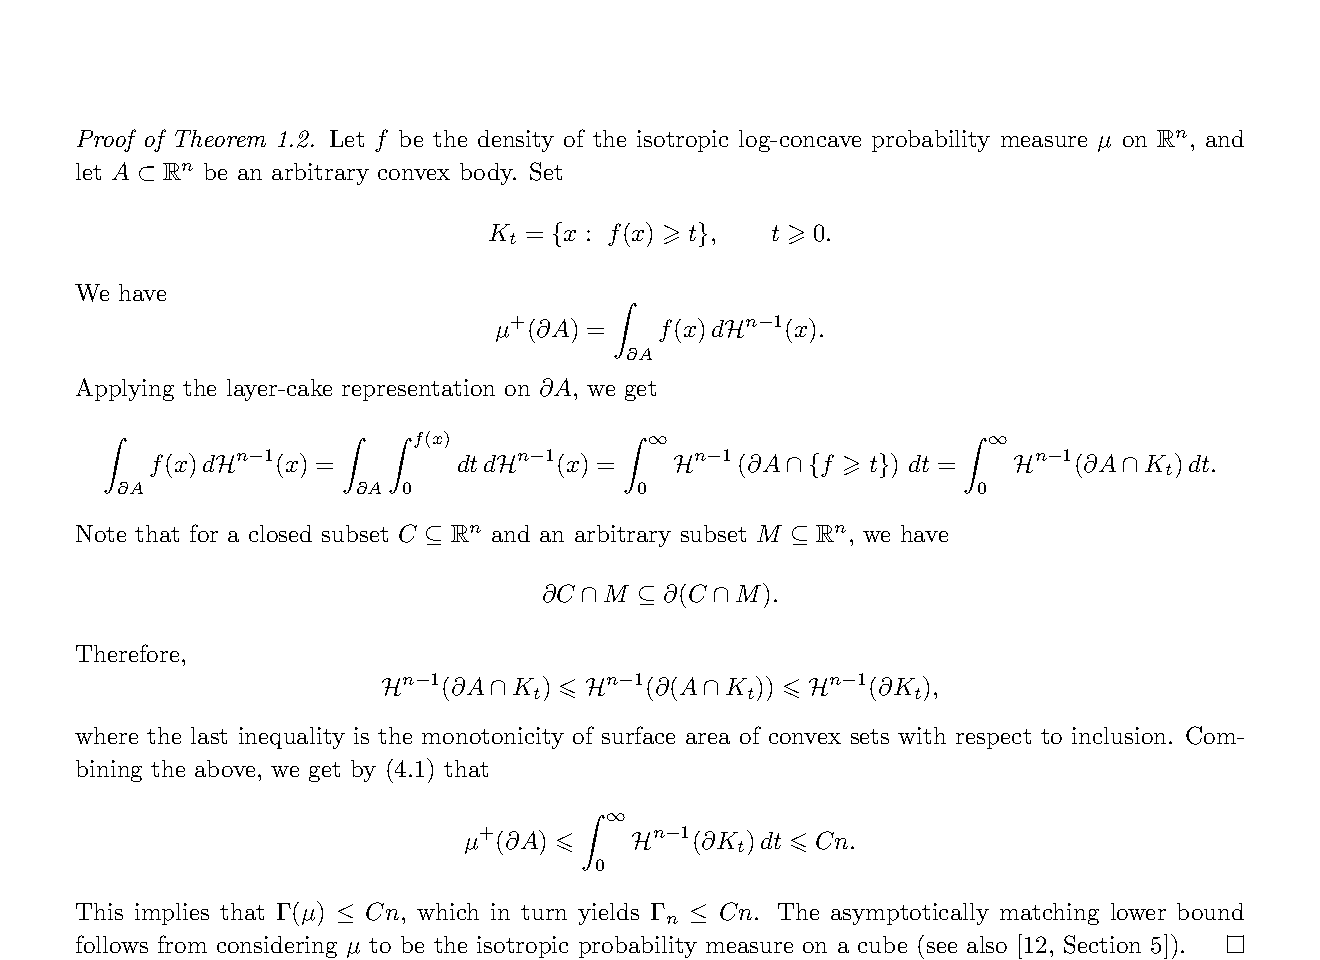
\includegraphics[width=0.88\textwidth]{figures/supporting_proof_crop.png}
\end{center}

\section*{Proof intuition}

The boundary of a test body can only meet each density level set along a
piece of boundary whose surface area is no larger than that of the whole
level set.  Layer cake sums these contributions over all density levels.
The difficult theorem in the later paper is precisely that the total surface
area of all levels is $O(n)$ for an isotropic log-concave density.  Once that
functional-perimeter estimate is available, every convex test body inherits
the same $O(n)$ bound at once.

\section*{Scope and provenance}

The identification is exact rather than merely implied: the later paper
names the same quantity, cites arXiv:2602.03831 for the preceding bound, and
states and proves the sharp order.  The source question occurs on page 4;
the later statement is Theorem 1.2 on page 3, and its short deduction is on
page 19.

The two bundled PDFs were reproducibly compiled, without source edits, from
the run's archived arXiv source downloads.  Their archive SHA-256 values are
\texttt{1eb7475c...d1339a} (2602.03831) and
\texttt{628e6a58...ec5a90} (2605.02747).  Exact rendered crops of the source
question, answer theorem, and proof are included above.

{\small
\textbf{References.}
[1] S. Brazitikos, A. Giannopoulos, A. Hmadi, and N. Tziotziou,
\emph{On the maximal perimeter of isotropic log-concave probability
measures}, arXiv:2602.03831 (2026).
[2] A. Eskenazis, A. Giannopoulos, and N. Tziotziou,
\emph{Functional perimeter and the dimensional Brunn--Minkowski inequality
for log-concave measures}, arXiv:2605.02747v2 (2026), Theorem 1.2 and
Section 4.
}

\end{document}
